\section{Modelado del Sistema}\label{sec:modelo}

En la Figura \ref{fig:statemachine}, se muestra el modelo del sistema que se va a
desarrollar como una m\'aquina de estados con cinco componentes
diferencidos:

\begin{itemize}
\item Las componentes BH1750 y DTH22 est\'an compuestas por dos
  estados: En \emph{S0} el sensor est\'a midiendo la magnitud f\'isica
  correspondiente y en \emph{S1} el sensor env\'ia los datos medidos
  al Arduino Uno al que est\'a conectado, volvi\'endose al estado
  \emph{S0} para comenzar una nueva medici\'on.
\item Los Arduinos Uno est\'an compuestos por tres estados: En
  \emph{S2} se reciben los datos del sensor, en \emph{S3} se procesan
  para mandarlos de manera unificada usando la estructura de datos
  Data (definida en Comm.h) y, finalmente, en \emph{S4} se env\'ian
  los datos a la Discovery, volviendo a esperar nuevos datos en
  \emph{S2}.
\item La Discovery SMT32 est\'a formada por tres estados: \emph{S5}
  espera a recibir datos de uno de los Arduinos. Una vez que los
  recibe, los procesa en el estado \emph{S6} y, finalmente, se produce
  la visualizaci\'on de los mismos en \emph{S7}. 
\end{itemize}

Este proyecto es un sistema completamente automatizado y, por lo
tanto, la interacci\'on con el usuario es inexistente. Esto lleva a
que no haya diagramas de casos de uso para el usuario. Por la misma
raz\'on, el diagrama de secuencia es completamente similar a lflujo de
eventos esperados por la m\'aquina de estados que define el sistema.
No obstante, durante la demo que se realice en clase, s\'i que habr\'a
interacci\'on, ya que se provocar\'a la variaci\'on de las magnitudes
f\'isicas medidas por los sensores involucrados en el proyecto.
\begin{center}
\begin{figure}[h]\label{fig:statemachine}
\hspace{3.5cm}
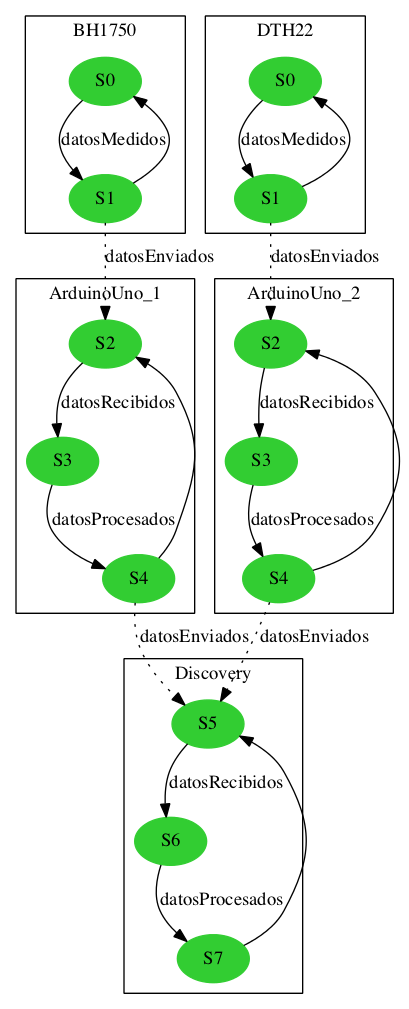
\includegraphics[scale=0.5]{images/maquina_estados.png}
\caption{M\'aquina de estados}
\end{figure}
\end{center}
